\documentclass[11pt]{report}
\usepackage[utf8]{inputenc}
\usepackage[margin=2.0cm]{geometry}
\usepackage{tikz}
\usepackage{fancyhdr}
\usepackage{xcolor}
\usepackage{minted}
\usepackage{graphicx}
\usepackage[parfill]{parskip}
\usepackage{lscape}
\usepackage{multirow}

\usetikzlibrary{automata, positioning, arrows, fit}

\title{Digital Engineering\\Project Task 2}
\author{Y3890959\\Y3878784}
\date{7th March 2023}

\pagestyle{fancy}
\fancyhead{}
\setlength{\headheight}{14pt}
\fancyhead[L]{Project Task 2}
\fancyhead[R]{Y3890959, Y3878784}
\fancyfoot{}
\fancyfoot[L]{Digital Engineering}
\fancyfoot[R]{\thepage}

\makeatletter
\let\ps@plain\ps@fancy 
\makeatother

\setminted {
    fontsize=\footnotesize,
    frame=single,
}

\begin{document}

\maketitle

\chapter*{Task 2: Clock domain crossing using dual-clock FIFOs}

\section*{1 - Description of FSMs}

\subsection*{SOURCE\_CTRL FSM}

\begin{figure}[h] % ’ht’ tells LaTeX to place the figure ’here’ or at the top of the page
    \centering % centers the figure
    \begin{tikzpicture}[->,>=stealth',shorten >=1pt,auto,node distance=7cm,semithick]
        \tikzstyle{every state}=[draw=none,text=black]

        \node[initial,state] (A)              {\textbf{IDLE}};;
        \node[state]         (B) [right of=A] {\textbf{COMP}};
        \node[state]         (C) [right of=B] {\textbf{HOLD}};

        \path (A) edge                         node[align=center, scale=0.8] {FROM\_OUTPUT = 0\\en = 1} (B)
              (B) edge [above, bend left=50]  node[align=center, scale=0.8] {FIFO\_FULL = 1} (C)
                  edge [above, bend right=50]  node[align=center, scale=0.8] {SWITCHES = COUNTER\\(or rst = 1)} (A)
              (C) edge                         node[align=center, scale=0.8] {FIFO\_FULL = 0} (B)
                  edge [above, bend left=50]   node[scale=0.8] {rst = 1} (A);
    \end{tikzpicture}
    \caption{SOURCE\_CTRL FSM state graph}
\end{figure}

The FSM starts at IDLE state, where all internal signals will reset and the LEDs are off. When the `en'
pushbutton is pressed and the output logic FSM has completed (FROM\_SOURCE goes low) the state goes to COMP
where the outputs are computed. As soon as `en' is toggled, when the FSM is still in IDLE, the values of the
SWITCHES is stored in a register `LIMT\_REG'. In the COMP state, the `LIMT\_CNT' is enabled and counts,
`EN\_SOURCE' also goes high so the outputs are computed, and the `FIFO\_WR\_EN' goes high so the values are
stored. When the FIFO becomes full, the SOURCE, counter, and FIFO\_WR\_EN are disabled, and the FSM goes to
HOLD state, where it stays until FIFO\_FULL becomes low again, then it goes back to COMP. The counter will
increment in the COMP state for every output computed and stored, once the counter value reaches the value
it signifies that the total number of outputs as set by the user via the SWITCHES has been computed, in this
case the FSM returns to the IDLE state. To make sure that the circuit doesn't break when the user changes the
SWITCHES mid-operation, the values of the SWITCHES is stored in `LIMT\_REG', and the logic will compare this.


\begin{landscape}
    \begin{table}
    \centering
    \resizebox{\columnwidth}{!}{%
    \begin{tabular}{|l|l|l|l|l|}
    \hline
    \textbf{STATE} & \textit{\textbf{EN\_SOURCE}} & \textit{\textbf{LIMT\_CNT\_EN}} & \textit{\textbf{LIMT\_CNT\_RST}} & \textit{\textbf{FIFO\_WR\_EN}} \\ \hline
    \multirow{2}{*}{IDLE} & 1 when en = 1 and FROM\_OUTPUT = 0 & \multirow{2}{*}{0}    & \multirow{2}{*}{1} & \multirow{2}{*}{0}    \\ \cline{2-2}
                          & 0 otherwise                        &                       &                    &                       \\ \hline
    \multirow{2}{*}{COMP} & 1 when FIFO\_FULL = 0              & 1 when FIFO\_FULL = 0 & \multirow{2}{*}{0} & 1 when FIFO\_FULL = 0 \\ \cline{2-3} \cline{5-5} 
                          & 0 otherwise                        & 0 otherwise           &                    & 0 otherwise           \\ \hline
    HOLD                  & 0                                  & 0                     & 0                  & 0                     \\ \hline
    \end{tabular}%
    }
    \caption{SOURCE\_CTRL FSM table of outputs}
    \end{table}
\end{landscape}





\subsection*{OUTPUT\_CTRL FSM}

\begin{figure}[h]
    \centering
    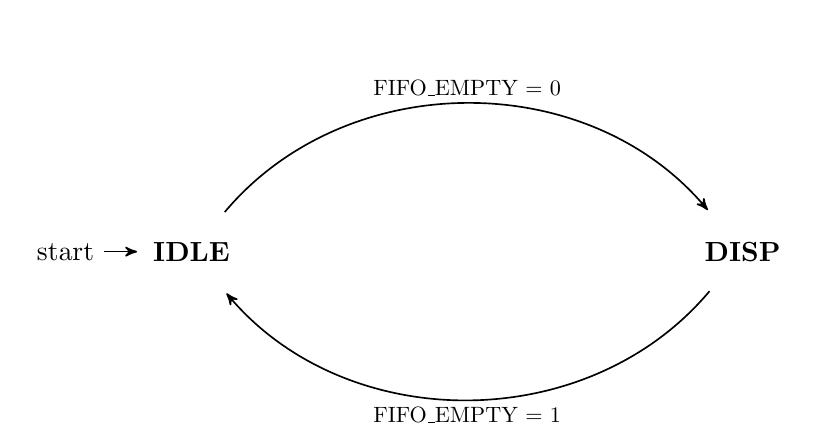
\begin{tikzpicture}[->,>=stealth',shorten >=1pt,auto,node distance=7cm,semithick]
        \tikzstyle{every state}=[draw=none,text=black]

        \node[initial,state] (A)              {\textbf{IDLE}};;
        \node[state]         (B) [right of=A] {\textbf{DISP}};

        \path (A) edge [above, bend left=50]  node[align=center, scale=0.8] {FIFO\_EMPTY = 0} (B)
              (B) edge [below, bend left=50]  node[align=center, scale=0.8] {FIFO\_EMPTY = 1} (A);
    \end{tikzpicture}
    \caption{OUTPUT\_CTRL FSM state graph}
\end{figure}

This FSM is quite simple and efficient with only two states, it completely ignores any user inputs via
switches and pushbuttons and only relies on whether the FIFO is empty or not. In the IDLE state, the delay
counter is disabled and reset and a 0 is output to `TO\_SOURCE', this is to tell the SOURCE logic that the
output logic is inactive. Once `FIFO\_EMPTY' goes low, the FSM goes to the DISP state. In the DISP state,
the `DISP\_CNT' counter is enabled (this is to add a delay where the LED outputs are held). As the FIFO is
set to the First-Word-Fall-Through mode, the `FIFO\_WR\_EN' needs to be high to pop the value at the end of
the delay, therefore that signal goes high as soon as the delay counter reaches the last value. The delay
counter will roll-over automatically. The LEDs will output the `DATA\_FROM\_FIFO' vector as long as the FIFO
is in DISP state.

\begin{landscape}
    \begin{table}
    \centering
    \resizebox{\columnwidth}{!}{%
    \begin{tabular}{|l|l|l|l|l|l|}
    \hline
    \textbf{STATE} &
      \textit{\textbf{DISP\_CNT\_EN}} &
      \textit{\textbf{DISP\_CNT\_RST}} &
      \textit{\textbf{TO\_SOURCE}} &
      \textit{\textbf{FIFO\_RD\_EN}} &
      \textit{\textbf{LEDs}} \\ \hline
    IDLE & 0 & 1 & 0 & 0           & 00 \\ \hline
    \multirow{2}{*}{DISP} &
      \multirow{2}{*}{1} &
      \multirow{2}{*}{0} &
      \multirow{2}{*}{1} &
      1 when DISP\_CNT\_OUT = disp\_delay-1 &
      \multirow{2}{*}{DATA\_FROM\_FIFO} \\ \cline{5-5}
         &   &   &   & 0 otherwise &    \\ \hline
    \end{tabular}%
    }
    \caption{OUTPUT\_CTRL FSM table of outputs}
    \end{table}
\end{landscape}





\section*{2 - VHDL Entity Code}
\subsection*{SOURCE\_CTRL}
\inputminted{vhdl}{../../../DE_Project_T2/DE_Project_T2.srcs/sources_1/imports/DigEng_Proj_T2_model/SOURCE_CTRL.vhd}

\newpage

\subsection*{OUTPUT\_CTRL}
\inputminted{vhdl}{../../../DE_Project_T2/DE_Project_T2.srcs/sources_1/imports/DigEng_Proj_T2_model/OUTPUT_CTRL.vhd}

\newpage

\section*{3 - VHDL Testbench Code}
\inputminted{vhdl}{../../../DE_Project_T2/DE_Project_T2.srcs/sim_1/imports/DigEng_Proj_T2_model/TOP_LEVEL_tb.vhd}

\newpage

\section*{3.1 Behavioural Simulation}

\subsection*{Waveform 1: Global Reset \& Initialisation Showing Output}
\begin{figure}[H]
    \includegraphics[width=\columnwidth]{Assets/Output_Reset.png}
\end{figure}

\subsection*{Waveform 2: Global Reset \& Initialisation Showing Source}
\begin{figure}[H]
       \includegraphics[width=\columnwidth]{Assets/Source_Reset.png}
\end{figure}

TEST 1: involves cycling through the first 5 values, this is the ensure that
all logic within this circuit is functioning properly.

\subsection*{Waveform 3: Test 1.1 }
\begin{figure}[H]
       \includegraphics[width=\columnwidth]{Assets/Test1_1.png}
\end{figure}

Zoomed out showing full cycle of first 5 values from btye `48' to `6C'.

\subsection*{Waveform 4: Test 1.2 }
\begin{figure}[H]
       \includegraphics[width=\columnwidth]{Assets/Test1_2.png}
\end{figure}

Waveform 4 shows the display counter incrementing from 0-29 as soon as `DISP\_CNT\_OUT' goes high. This ensures that the
LED's flash a value for a second at a time.

\subsection*{Waveform 5: Test 1.3 }
\begin{figure}[H]
       \includegraphics[width=\columnwidth]{Assets/Test1_3.png}
\end{figure}

Waveform 5 shows the source state entering `COMP' mode and storing the value of the switches so that a change mid 
operation doesn't affect the circuit\\

TEST 2: Following from Test 1, once the last byte has been output, we need to verify that the LEDs output zeros.

\subsection*{Waveform 6: Test 2 }
\begin{figure}[H]
       \includegraphics[width=\columnwidth]{Assets/Test2.png}
\end{figure}

Above waveform shows that the output returns to 0 after a full cycle.\\

TEST 3: Following from TEST 1, a reset will be inputted via the push-button. This is the verify that the circuit resets
properly and goes back to the initial state.

\subsection*{Waveform 7: Test 3.1 }
\begin{figure}[H]
       \includegraphics[width=\columnwidth]{Assets/Test3_1.png}
\end{figure}

Above shows output signals being reset after operation.

\subsection*{Waveform 8: Test 3.2 }
\begin{figure}[H]
       \includegraphics[width=\columnwidth]{Assets/Test3_2.png}
\end{figure}

Above shows source signals being reset after operation.\\

TEST 4: Cycle through the first 5 values just like in TEST 1, but the enable button will be pressed while the logic is in
operation (after the 1st input). This test will verify that the enable input will be ignored.

\subsection*{Waveform 9: Test 4 }
\begin{figure}[H]
       \includegraphics[width=\columnwidth]{Assets/Test4.png}
\end{figure}

Above shows enable pressed mid-operation the value of `LMT\_REG\_OUT' changes to 5 for one clock cycle then returns back to zero. 
This is the expected output as you can see that the source state never changes from idle.\\ 

TEST 5: Continue from TEST 4, the reset button will be toggled after the 4th input, this will verify that the circuit can be reset
while the FSM is in operation.

\subsection*{Waveform 10: Test 5 }
\begin{figure}[H]
       \includegraphics[width=\columnwidth]{Assets/Test5.png}
\end{figure}

Waveform 10 shows a reset mid way through operation. The state goes back to idle and the LED outputs zeros.\\

TEST 6: Cycle through the first 5 values just like in TEST 4, but the switches will be changed while the FSM is operation
(after the 2nd input). This test will verify that changing the switches will be ignored when the FSM is in operation.

\subsection*{Waveform 11: Test 6 }
\begin{figure}[H]
       \includegraphics[width=\columnwidth]{Assets/Test6.png}
\end{figure}

Waveform 11 shows that changing the switch value from 5 to 3 doesn't have any effect on the output\\

TEST 7: Cycle through as many inputs as it takes to cause the FIFO to become full, verify that the circuit can still function
as designed and handle the FIFO becoming full.

\subsection*{Waveform 12: Test 7.1 }
\begin{figure}[H]
       \includegraphics[width=\columnwidth]{Assets/Test7_1.png}
\end{figure}

Shows full cycle from source side\\

\subsection*{Waveform 13: Test 7.2 }
\begin{figure}[H]
       \includegraphics[width=\columnwidth]{Assets/Test7_2.png}
\end{figure}

Shows the source state going into hold after `FIFO\_FULL' goes to logic high,

\subsection*{RTL Component Statistics}
\inputminted[firstline=165,lastline=190]{text}{../../../DE_Project_T2/DE_Project_T2.runs/synth_1/TOP_LEVEL.vds}

\newpage

\subsection*{RTL Hierarchical Component Statistics}
\inputminted[firstline=193,lastline=264]{text}{../../../DE_Project_T2/DE_Project_T2.runs/synth_1/TOP_LEVEL.vds}


\end{document}
